\documentclass[12pt, a4paper]{report}

\usepackage{titlesec}
\usepackage[plain]{fullpage}
\usepackage{titling}
\usepackage{geometry}
\usepackage{graphicx}
\usepackage{fancyhdr}

\renewcommand{\maketitle}{
  \begin{center}

  \vspace*{\fill}
  {\huge\bfseries\thetitle}\\
  \vspace{1.2em}
  {\large\bfseries\theauthor}
  \vspace*{\fill}
  \end{center}

  \newpage
}

\renewcommand{\rmdefault}{ptm}

\renewcommand*\contentsname{
  \begin{center}
    \huge\bfseries{Sumário}
  \end{center}
}

\renewcommand*\chaptername{Capítulo}


\title{Free Open Source Software\\\LARGE\vspace{0.5em} Software livre e de código aberto, licenças e história.}
\author{Raimundo Nonato Dos Santos Junior}

\begin{document}

\pagenumbering{gobble}

\maketitle

\tableofcontents

\chapter{O começo do movimento de software livre}

\section{Introdução}

\pagenumbering{arabic}

Open Source é uma dos movimentos da área de desenvolvimento de software mais importantes do momento, onde ter uma conta em um serviço de hospedagem de códigos como Github e colaborar em projetos de código aberto são fatores que podem te ajudar a ingressar no mercado de trabalho, por ser uma ótima forma de se destacar para empresas, que buscam justamente esse perfil e valorizam essa cultura de compartilhamento e colaboração, porém esse conceito não é novo e vem de várias
A ideia de colaboração entre programadores não é um conceito novo, os primeiros desenvolvedores e hackers do período até 1970, tinham isso como norma.
A avanço tecnológico e mudanças fizeram que os computadores, e claro, o software que eles carregavam formas de 

\section{História}

Nos anos de 1970, os desenvolvedores de software e hackers formavam uma comunidade em volta do compartilhamento de software. Após as grandes mudanças no mundo da informática em 1980, e os computares pessoais se tornarem mais acessíveis, os programadores e empresas da época viram como oportunidade de gerar lucro para si mesmos a produção de software de código fechado, onde era necessário pagar algum tipo de taxa pelo acesso ao software. Os programas proprietários tinham dominado completamente o cenário.

Richard Stallman viu todo o desenrolar dessa história dos laboratórios de Inteligência artificial do MIT, e decidiu que não se tornaria parte dessa mudança. 

\section{Richard Stallman}

\begin{center}
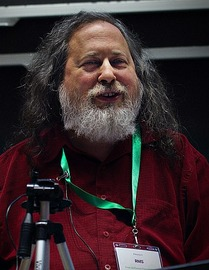
\includegraphics[]{imgs/richard_stallman.jpg}
\end{center}

É o fundador do movimento de software livre e do sistema operacional GNU.

\chapter{Software Livre}

\section{O Sistema Operacional GNU}

O Sistema Operacional GNU foi desenvolvido por Richard Stallman (rms) em 1983 como um sistema 100\% livre, que daria o controle aos usuários.

\section{GNU General Public License}

A Licença GNU General Public License (ou GNU GPL) é a licença usada pelos programas GNU e vários outros softwares livres.
A GNU GPL é uma licença copyleft feita essencialmente para garantir que um programa permanecesse livre e não pudesse ser tornado em software proprietário.

\section{Free Software Foundation}

A Free Software Foundation (FSF) foi criada em 1985, inicialmente para arrecadar fundos para o sistema operacional GNU. A FSF promove a liberdade dos usuários de computador promovendo o desenvolvimento de software e documentação livre e luta contra tecnologias como Digital Restrictions Management (DRM) e patentes de software.

\section{Definição de software livre}

De acordo com a Free Software Foundation, a definição de software livre (free software) é de um programa de computador que respeite as liberdades do usuário e comunidade, o que significa que os usuários precisam ter a liberdade de executar, copiar, distribuir, estudar, mudar e melhorar o programa. Portanto é importante entender que o software livre não é sobre preço, mas sobre liberdade dos usuários.

Um programa é considerado livre se o programa respeita as 4 liberdades essenciais dos usuários:

\begin{itemize}

  \item{A liberdade de executar o programa como você desejar, para qualquer propósito (liberdade 0).}
  \item{A liberdade de estudar como o programa funciona, e modificar ele de forma que faça seus processamentos da forma que deseja (liberdade 1).Acesso ao código fonte é um pré-requisito para isto.}
  \item{A liberdade de redistribuir copias assim você pode ajudar outros (liberdade 2).}
  \item{A liberdade de distribuir cópias da sua versão modificada para outros (liberdade 3). Ao fazer isso você pode dar a toda comunidade a possibilidade de beneficiar-se das suas mudanças. Acesso ao código fonte é um pré-requisito para isto.}

\end{itemize}

\chapter{Software de código aberto}

\section{História}

No final da década de 1990, com a liberação do código fonte do navegador Netscape e o reconhecimento pela mídia mainstream do Linux fez com que o interesse pelo desenvolvimento de software colaborativo crescesse mais.

\section{Open Source Iniciative}

A Open Source Iniciative (OSI) foi criada em 1998 como uma organização educacional, que 

\section{Definição de software de código aberto}

\begin{enumerate}

  \item{Distribuição Livre}

    A licença não deve restringir a venda ou distribuição do software como um componente de um conjunto de softwares contendo aplicações de diversas fontes. As licenças não devem requerer uma permissão ou pagamento pela venda.

  \item{Código fonte}

    O programa deve incluir o código fonte, e deve permitir a distribuição do código fonte também de forma copilada. Onde um produto não for distribuído com o código fonte, deve haver uma meios de obter o código fonte devidamente publicados por não mais que um razoável preço de reprodução, de preferência através de download via internet sem encargos. O código fonte deve ser preferido da forma em que o programador modificará o programa. Deliberadamente obscurecendo o código fonte não é permitido. Formas intermediárias como uma saída de um preprocessador de texto ou tradutor não são permitidas.

  \item{Trabalhos derivados}

    A licença deve permitir modificações e trabalhos derivados, e deve permitir eles de ser distribuídos nos mesmos termos da licença do programa original.

  \item{Integridade do código fonte do autor}

    A licença pode restringir o código fonte de ser distribuído de forma modificada \emph{somente se} a licença permite a distribuição de "arquivos de patch" com o código fonte para o propósito de modificar o programa no buid time. A licença deve explicitamente permitir a distribuição de software construído da versão modificada do código fonte. A licença pode requerer que trabalhos derivados tenham nomes ou números de versões diferentes do programa original.

  \item{Nenhuma discriminação contra pessoas ou grupos}

    A licença não deve discriminar nenhum indivíduo ou grupo de pessoas.

  \item{Nenhuma discriminação contra campos específicos}

    A licença não deve restringir ninguém de fazer o uso de programa em qualquer campo. Por exemplo, o programa não pode ser restringido de ser usado em um negócio, ou de ser usado para pesquisa genética.

  \item{Distribuição da licença}

    Os direitos atribuídos ao programa devem ser aplicados para todos aqueles que o programa é redistribuído sem a necessidade da execução de uma licença adicional.

  \item{Licença não deve ser específica para um produto}

    Os direitos atribuídos a um programa não devem ser dependentes do programa ser uma parte de uma distribuição de software específica. Se o programa é extraído daquela distribuição e usado ou distribuído dentro dos termos da licença do programa, todos os envolvidos para qual o programa é redistribuído deve ter os mesmos direitos daqueles que garantiram em conjunção com a distribuição do software original.

  \item{Licenças não devem restringir outros softwares}

    A licença não deve restringir outros softwares que são distribuídos jutos com o software licenciado. Por exemplo, a licença não deve insistir que todos os outros programas distribuídos sobre a mesma plataforma sejam software de código aberto.

  \item{Licença deve ser neutra a tecnologia}

      Nenhuma cláusula da licença pode ser definida para qualquer tecnologia específica ou estilo de interface.

\end{enumerate}

\chapter{Licenças}

\section{O que é uma licença}

\section{Licenças de Software}

\section{Copyleft}

Enquanto o copyright protege os direitos dos autores restringindo o direito de cópia, o conceito de copyleft, que não é exclusivo de licenças de software, é que qualquer peça licenciada, precisa ser licenciada nos mesmos termos. Falando de licenças, a GNU GPL (General Public License) é um exemplo de licença copyleft, porque obriga que as versões modificadas do software licenciado também siga as mesmas diretrizes, impedindo versões fechadas de softwares licenciados com ela.

\section{Licenças permissivas e licenças restritivas}


Quando falamos de licenças, outras categorias de licença são as licenças permissivas e restritivas:

\begin{itemize}

\item Licenças Permissivas: Têm pouquíssimas restrições, e são muitas vezes chamadas de licenças estilo BSD, onde BSD, ou suas variantes que é o caso mais comum, seguem esse padrão.

\item Licenças restritivas: que com o objetivo de garantir a liberdade dos usuários, tira poder dos desenvolvedores, e tem mais restrições. Também são chamadas de licença copyleft.

\end{itemize}

\chapter{Programas FOSS}

\section{Onde estão os programas FOSS?}

\subsection{GNU/Linux}

Licença: GPL

\subsubsection{Debian}

Contrato Social (Social contract) 

\subsubsection{Todas as distribuições Linux são livre?}

De acordo com a GNU (e portanto Free Software Foundation), a resposta é não. Os padrões que determinam um sistema GNU/Linux ser livre em sua definição são:


\chapter{Perguntas e Respostas}

\section{Perguntas}

\subsection{Introdução}

\begin{enumerate}

  \item Você sabe o que é software de código livre? 

  \item Você sabe o que é software de código aberto? 

  \item Você usa algum software livre ou de código aberto? 

\end{enumerate}

\subsection{Programas FOSS}

\begin{enumerate}

  \item Você usa ou já usou algum sistema GNU/Linux? 

  \item Site o nome de qualquer sistema GNU/Linux que você já utilizou. 

  \item Você acha que todo sistema Linux é um sistema livre? 

\end{enumerate}


\end{document}
